%!Mode:: "TeX:UTF-8"
\documentclass[a4paper,11pt,UTF8]{ctexart}

\usepackage{indentfirst} %缩进
\usepackage{xeCJK}    %使用系统字体
\usepackage{fancyhdr} %自定义页眉页脚
\pagestyle{plain}                   %不设置页眉页脚
\usepackage{amsmath, amsthm, amssymb, amsfonts} %数学公式
\usepackage[a4paper,left=3cm,right=3cm,top=3cm,bottom=3cm]{geometry}
%\usepackage[tmargin=1in,bmargin=1in,lmargin=1.25in,rmargin=1.25in]{geometry}.
\usepackage{booktabs} %插入表格
\usepackage[section]{placeins} %避免浮动
\usepackage{listings} %插入代码
\usepackage{ctex}     %中文宏包
\usepackage{bm}
\usepackage[svgnames, table]{xcolor} %彩色表格
\usepackage{algorithm}          %伪代码
\usepackage{algorithmicx}
\usepackage{algpseudocode}
\usepackage{algorithm,algpseudocode,float}
\usepackage{lipsum}
\usepackage{enumitem}           %调整列举环境
\usepackage{hyperref}
\hypersetup{
    colorlinks=true,
    linkcolor=blue,
    filecolor=blue,      
    urlcolor=blue,
    citecolor=cyan,
}
\usepackage{fontspec,xunicode}
\defaultfontfeatures{Mapping=tex-text} %如果没有它,会有一些 tex 特殊字符无法正常使用,比如连字符。

\usepackage{graphicx}
\graphicspath{{imgs/}}

%%%%%%%%%%%%%%%%%%%%%%%%%%%%%%%%%%%%%%%%%%%%%%%%%%%%%%%%%%%%%%%%
% 缩进及行间距
%%%%%%%%%%%%%%%%%%%%%%%%%%%%%%%%%%%%%%%%%%%%%%%%%%%%%%%%%%%%%%%%
\setlength{\parindent}{22pt} %重新定义缩进长度
\setlength{\baselineskip}{20pt}  %定义行间距
%\renewcommand{\baselinestretch}{1.1} %定义行间距

%%%%%%%%%%%%%%%%%%%%%%%%%%%%%%%%%%%%%%%%%%%%%%%%%%%%%%%%%%%%%%%%
% 列表设置
%%%%%%%%%%%%%%%%%%%%%%%%%%%%%%%%%%%%%%%%%%%%%%%%%%%%%%%%%%%%%%%%
\setenumerate{fullwidth,itemindent=\parindent,listparindent=\parindent,itemsep=0ex,partopsep=0pt,parsep=0ex}
\setenumerate[2]{label=\alph*),leftmargin=1.5em}  %二级item设置
\setitemize{itemindent=38pt,leftmargin=0pt,itemsep=-0.4ex,listparindent=26pt,partopsep=0pt,parsep=0.5ex,topsep=-0.25ex}
\setdescription{itemindent=38pt,leftmargin=0pt,itemsep=-0.4ex,listparindent=26pt,partopsep=0pt,parsep=0.5ex,topsep=-0.25ex}

%%%%%%%%%%%%%%%%%%%%%%%%%%%%%%%%%%%%%%%%%%%%%%%%%%%%%%%%%%%%%%%%
% 图的标题行间距设置
%%%%%%%%%%%%%%%%%%%%%%%%%%%%%%%%%%%%%%%%%%%%%%%%%%%%%%%%%%%%%%%%
\newcommand{\bottomcaption}{%
\setlength{\abovecaptionskip}{6pt}%
\setlength{\belowcaptionskip}{6pt}%
\caption}


%%%%%%%%%%%%%%%%%%%%%%%%%%%%%%%%%%%%%%%%%%%%%%%%%%%%%%%%%%%%%%%%
% 字体定义
%%%%%%%%%%%%%%%%%%%%%%%%%%%%%%%%%%%%%%%%%%%%%%%%%%%%%%%%%%%%%%%%
% \setmainfont{Times New Roman}  %默认英文字体.serif是有衬线字体sans serif无衬线字体
\setmonofont{Consolas}
\setCJKmainfont[ItalicFont={楷体}, BoldFont={黑体}]{宋体}%衬线字体 缺省中文字体为
\setCJKsansfont{黑体}
\punctstyle{hangmobanjiao}
%-----------------------xeCJK下设置中文字体------------------------------%
\setCJKfamilyfont{song}{SimSun}                             %宋体 song
\newcommand{\song}{\CJKfamily{song}}
\setCJKfamilyfont{fs}{FangSong}                      %仿宋  fs
\newcommand{\fs}{\CJKfamily{fs}}
\setCJKfamilyfont{ktgb}{KaiTi}                      %楷体2312 ktgb
\newcommand{\ktgb}{\CJKfamily{ktgb}}
\setCJKfamilyfont{yh}{Microsoft YaHei}                    %微软雅黑 yh
\newcommand{\yh}{\CJKfamily{yh}}
\setCJKfamilyfont{hei}{SimHei}                              %黑体  hei
\newcommand{\hei}{\CJKfamily{hei}}
\setCJKfamilyfont{hwxk}{STXingkai}                                %华文行楷  hwxk
\newcommand{\hwxk}{\CJKfamily{hwxk}}
%------------------------------设置字体大小------------------------%
\newcommand{\shiyanbaogao}{\fontsize{36pt}{\baselineskip}\selectfont}
\newcommand{\chuhao}{\fontsize{42pt}{\baselineskip}\selectfont}     %初号
\newcommand{\xiaochuhao}{\fontsize{36pt}{\baselineskip}\selectfont} %小初号
\newcommand{\yihao}{\fontsize{28pt}{\baselineskip}\selectfont}      %一号
\newcommand{\erhao}{\fontsize{21pt}{\baselineskip}\selectfont}      %二号
\newcommand{\xiaoerhao}{\fontsize{18pt}{\baselineskip}\selectfont}  %小二号
\newcommand{\sanhao}{\fontsize{15.75pt}{\baselineskip}\selectfont}  %三号
\newcommand{\sihao}{\fontsize{14pt}{\baselineskip}\selectfont}       %四号
\newcommand{\xiaosihao}{\fontsize{12pt}{\baselineskip}\selectfont}  %小四号
\newcommand{\wuhao}{\fontsize{10.5pt}{\baselineskip}\selectfont}    %五号
\newcommand{\xiaowuhao}{\fontsize{9pt}{\baselineskip}\selectfont}   %小五号
\newcommand{\liuhao}{\fontsize{7.875pt}{\baselineskip}\selectfont}  %六号
\newcommand{\qihao}{\fontsize{5.25pt}{\baselineskip}\selectfont}    %七号

%%%%%%%%%%%%%%%%%%%%%%%%%%%%%%%%%%%%%%%%%%%%%%%%%%%%%%%%%%%%%%%%
% 图题字体大小相同
%%%%%%%%%%%%%%%%%%%%%%%%%%%%%%%%%%%%%%%%%%%%%%%%%%%%%%%%%%%%%%%%
\usepackage{caption}
\captionsetup{font={footnotesize}}   % footnotesize = 9pt
\captionsetup[lstlisting]{font={footnotesize}}

%%%%%%%%%%%%%%%%%%%%%%%%%%%%%%%%%%%%%%%%%%%%%%%%%%%%%%%%%%%%%%%%
% 重定义枚举编号为 1),2)...
%%%%%%%%%%%%%%%%%%%%%%%%%%%%%%%%%%%%%%%%%%%%%%%%%%%%%%%%%%%%%%%%
\renewcommand{\labelenumi}{\theenumi)}


%%%%%%%%%%%%%%%%%%%%%%%%%%%%%%%%%%%%%%%%%%%%%%%%%%%%%%%%%%%%%%%%
% 重定义section标题
%%%%%%%%%%%%%%%%%%%%%%%%%%%%%%%%%%%%%%%%%%%%%%%%%%%%%%%%%%%%%%%%
\CTEXsetup[format={\sihao\CJKfamily{zhhei}\zihao{4}},number={\chinese{section}},name={,、~},aftername={},indent={0pt},beforeskip={6pt},afterskip={6pt},format+={\flushleft}]{section}
\CTEXsetup[format={\Large\bfseries\CJKfamily{zhkai}\zihao{4}},name={(,)},number={\chinese{subsection}},aftername={},indent={22pt},beforeskip={14pt},afterskip={2pt}]{subsection}
\CTEXsetup[number={\chinese{section}},name={附录, ~~ }]{appendix}



%%%%%%%%%%%%%%%%%%%%%%%%%%%%%%%%%%%%%%%%%%%%%%%%%%%%%%%%%%%%%%%%
% 标题名称中文化
%%%%%%%%%%%%%%%%%%%%%%%%%%%%%%%%%%%%%%%%%%%%%%%%%%%%%%%%%%%%%%%%
\renewcommand\figurename{\hei 图}
\renewcommand\tablename{\hei 表}
\renewcommand\lstlistingname{\hei 代码}
\renewcommand{\algorithmicrequire}{\textbf{输入:}}
\renewcommand{\algorithmicensure}{\textbf{输出:}}
\newtheorem{define}{定义}

%%%%%%%%%%%%%%%%%%%%%%%%%%%%%%%%%%%%%%%%%%%%%%%%%%%%%%%%%%%%%%%%
% 代码设置
%%%%%%%%%%%%%%%%%%%%%%%%%%%%%%%%%%%%%%%%%%%%%%%%%%%%%%%%%%%%%%%%
\lstset{
 columns=fixed,
 numbers=left,                                        % 在左侧显示行号
 numberstyle=\tiny\color{gray},                       % 设定行号格式
 frame=single,                                        % 单线背景边框
 breaklines=true,                                     % 设定LaTeX对过长的代码行进行自动换行
 keywordstyle=\color[RGB]{40,40,255},                 % 设定关键字颜色
 numberstyle=\footnotesize\color{darkgray},
 commentstyle=\it\color[RGB]{0,96,96},                % 设置代码注释的格式
 stringstyle=\rmfamily\slshape\color[RGB]{128,0,0},   % 设置字符串格式
 showstringspaces=false,                              % 不显示字符串中的空格
 language=java,                                        % 设置语言
 basicstyle=\linespread{1.0}\xiaowuhao\ttfamily,                      % 字体字号
 %lineskip=10pt,
 %baselinestretch=1,
}

%%%%%%%%%%%%%%%%%%%%%%%%%%%%%%%%%%%%%%%%%%%%%%%%%%%%%%%%%%%%%%%%
% 伪代码分页
%%%%%%%%%%%%%%%%%%%%%%%%%%%%%%%%%%%%%%%%%%%%%%%%%%%%%%%%%%%%%%%%
\makeatletter
\renewcommand{\ALG@name}{算法}
\newenvironment{breakablealgorithm}
  {% \begin{breakablealgorithm}
   \begin{center}
     \refstepcounter{algorithm}% New algorithm
     \hrule height.8pt depth0pt \kern2pt% \@fs@pre for \@fs@ruled
     \renewcommand{\caption}[2][\relax]{% Make a new \caption
       {\raggedright\textbf{\ALG@name~\thealgorithm} ##2\par}%
       \ifx\relax##1\relax % #1 is \relax
         \addcontentsline{loa}{algorithm}{\protect\numberline{\thealgorithm}##2}%
       \else % #1 is not \relax
         \addcontentsline{loa}{algorithm}{\protect\numberline{\thealgorithm}##1}%
       \fi
       \kern2pt\hrule\kern2pt
     }
  }{% \end{breakablealgorithm}
     \kern2pt\hrule\relax% \@fs@post for \@fs@ruled
   \end{center}
  }
\makeatother



\begin{document}
\xiaosihao\song

\begin{titlepage}
\center{\yihao{\hei{机器学习课程实验报告}}}
\vspace{6cm}
\center{\erhao{\ktgb{逻辑回归}}}
\vspace{4cm}

\begin{center}
\begin{large}
\begin{tabular}{rc}
\xiaoerhao{\hei{学\qquad 号}}& \hspace{1.7cm}\xiaoerhao{\hei{1180301007\hspace{1.7cm}}} \\
\cline{2-2}\\
\xiaoerhao{\hei{姓\qquad 名}}& \xiaoerhao{\hei{赵锦涛}}\\
\cline{2-2}\\
\xiaoerhao{\hei{实验时间}}& \xiaoerhao{\hei{2020年10月}}\\
\cline{2-2}
\end{tabular}
\end{large}
\end{center}
\vfill \hfill
\end{titlepage}
\clearpage


\setlength{\parskip}{6pt}  %定义段间距

\section{实验目的:}
理解逻辑回归模型,掌握逻辑回归模型的参数估计算法。
\section{实验要求:}
实现两种损失函数的参数估计(1,无惩罚项;2.加入对参数的惩罚),可以采用梯度下降、共轭梯度或者牛顿法等。	
\section{实验环境:}
Python 3.8, Windows 10
\section{实验原理:}
逻辑回归是一种分类方法。对于二分类问题,给定输入$X = <X_{1}, ... , X_{n}>$,输出$Y \in \{0,1\}$,有
$$P(Y = 1 | X) = \frac{exp(w \cdot X + b)}{1 + exp(w \cdot X + b)}$$
$$P(Y = 0 | X) = \frac{1}{1+exp(w \cdot X + b)} $$
扩充$X$向量为$X = \{1, X_{1}, ... ,X_{n}\}$,$w$向量为$w = \{b, w_{1}, ... , w_{n}\}$,则后验类概率可表示为
$$P(Y = 1 | X) = \frac{exp(w \cdot X)}{1 + exp(w \cdot X)}$$
$$P(Y = 0 | X) = \frac{1}{1+exp(w \cdot X)} $$
当训练得到参数$w$后,便可将样本代入求得相应的概率,样本分类类别取使概率较大的那类。 \par
逻辑回归模型参数估计时可使用最大似然法估计方法参数,设
$$P(Y = 1 | x) = p(x), P(Y = 0 | x) = 1 - p(x)$$
似然函数为
$$\prod [p(x_{i})]^{y_{i}}[1-p(x_{1})]^{1 - y_{i}}$$
取对数有
\begin{equation}  
  \begin{aligned}
    L(w) &= \sum [y_{i}lnp(x_{i}) + (1 - y_{i})ln(1-p(x_{i}))] \\
    &= \sum[y_{i}(w\cdot x_{i}) - ln(1 + exp(w \cdot x_{i}))] \nonumber
  \end{aligned}
\end{equation}
相应的平均对数似然损失函数为(其中N为数据集大小)
$$ J(w) = - \frac{1}{N}L(w)$$
该函数为一个下凸函数,最小化损失函数可以通过梯度下降法来求解。计算梯度有:
$$ \frac{\partial J(w)}{\partial w_{j}} = \frac{1}{N}\sum_{i = 1}^{N}(p(x_{i}) - y_{i})x_{i}^{j}$$
所以参数的迭代过程为
$$w_{j} := w_{j} - \alpha \frac{1}{N} \sum_{i = 1}^{N}(p(x_{i}) - y_{i})x_{i}^{j}$$
设sigmoid函数$$ sigmoid(x) = \frac{1}{1 + e^{-x}}$$
输入矩阵为
$$
X = \begin{bmatrix}
1 & x_{1}^{1} & \cdots & x_{1}^{m} \\
1 & x_{2}^{1} & \cdots & x_{2}^{m} \\
\vdots & \vdots & \ddots & \vdots \\
1 & x_{n}^{1} & \cdots & x_{n}^{n}
\end{bmatrix}
$$
其中每行代表一个样本,这些样本所对应的类别向量$Y = [y_{1}, y_{2}, ... ,y_{n}]^{T}$,参数向量$ \bm{w} = [w_{0}, w_{1}, ..., w_{m}]^{T}$
所以参数迭代过程的矩阵表示为
$$ \bm{w}_{i+1} = \bm{w} _{i} - \alpha \frac{1}{N} X^{T}(sigmoid(X\bm{w}_{i}) - Y)$$
根据贝叶斯定理
$$p(\bm{w} | \mathcal{D}) = \frac{p( \mathcal{D} | \bm{w})p(\bm{w})}{p(\mathcal{D})} $$
有
$$ posterior \propto likelihood \times prior$$
根据最大后验准则,给模型加入正则项,此时损失函数变为
$$ J(w) = - \frac{1}{N}(\sum [y_{i}lnp(x_{i}) + (1 - y_{i})ln(1-p(x_{i}))] + \frac{ \lambda }{2}w^{T}w)$$
参数的迭代过程变为
$$w_{j} := (1 - \alpha \frac{\lambda}{N})w_{j} - \alpha \frac{1}{N} \sum_{i = 1}^{N}(p(x_{i}) - y_{i})x_{i}^{j}$$
矩阵迭代形式为
$$ \bm{w}_{i+1} = (1 - \alpha \frac{\lambda}{N})\bm{w} _{i} - \alpha \frac{1}{N} X^{T}(sigmoid(X\bm{w}_{i}) - Y)$$

\section{代码实现}
本次实验共有7个文件,其名称和作用分别为:
\begin{itemize}
  \item \emph{datagen.py} \quad 生成训练数据
  \item \emph{calcacc.py} \quad 计算精度
  \item \emph{loss.py} \quad 计算损失函数
  \item \emph{plot.py} \quad 绘制图表
  \item \emph{gradient.py} \quad 梯度下降法
  \item \emph{uci.py} \quad 对UCI数据集进行预处理
  \item \emph{uci\_gradient.py} \quad 对预处理后的UCI数据使用梯度下降法进行训练
\end{itemize}
在本次实验中,自主生成的数据样本共有四个维度,满足贝叶斯假设条件下,各维度符合高斯分布,其均值分别为$1,2,3,4$,方差均为$0.2$。不满足贝叶斯假设条件下,各维度的协方差矩阵为
$$Cov = \begin{bmatrix}
0.2 & 0.1 & 0.1 & 0.1 \\
0.1 & 0.2 & 0.1 & 0.1 \\
0.1 & 0.1 & 0.2 & 0.1 \\
0.1 & 0.1 & 0.1 & 0.2
\end{bmatrix}$$
分类规则为当样本各维度的和大于10时分为正类,否则为负类。
UCI数据集使用的是haberman数据集,具体信息请见\href{https://archive.ics.uci.edu/ml/datasets/Haberman%27s+Survival}{Haberman's Survival Data Set}
\section{实验结果与分析}
\subsection{数据集大小}
实验过程中,使用了不同大小的数据集进行测试。训练集的样本大小分别为20和100,测试集的样本大小为100,学习率为0.1,各运行20次,计算其精度,结果如图一所示。
\begin{figure}[htbp]
  \centering
  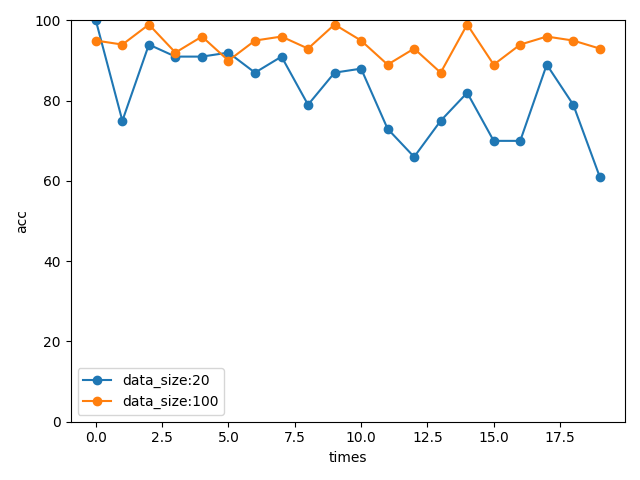
\includegraphics[width=0.6\textwidth]{img_1.png}
  \bottomcaption{data\_size = 20, data\_size = 100}
\end{figure}
可以看出,训练集大小为20的时候,测试结果较差,出现了欠拟合现象。提高样本数量至100后,能够较好地提高模型预测的精度,解决了欠拟合的问题。
\subsection{正则项}
图二为加入正则项和不加入正则项的实验结果对比。其中,训练样本个数均为30,正则化项系数为0.0008。可以发现,加入正则项后,整体而言精度有所提高,但其效果不如增加训练样本,这可能和正则化项系数的选择有关。
\begin{figure}[htbp]
  \centering
  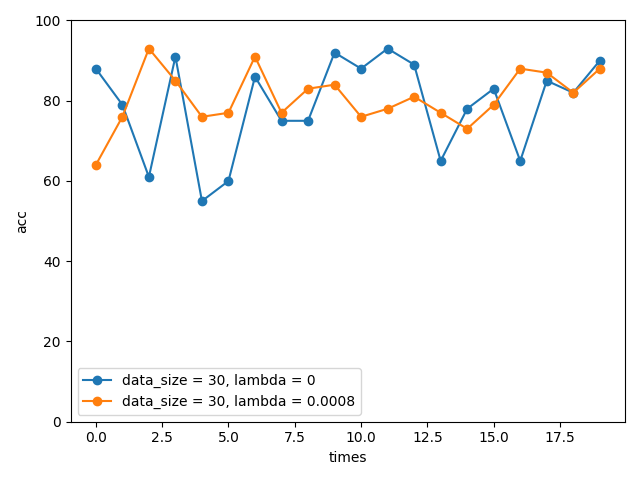
\includegraphics[width=0.6\textwidth]{img_2.png}
  \bottomcaption{加入正则化项}
\end{figure}
\subsection{贝叶斯假设}
实验中使用了满足贝叶斯假设的数据和不满足贝叶斯假设的数据进行测试,其训练样本个数均为50,可以发现两者效果相近,都比较好。逻辑回归方法也能对不满足贝叶斯假设的数据进行良好分类。
\begin{figure}[htbp]
  \centering
  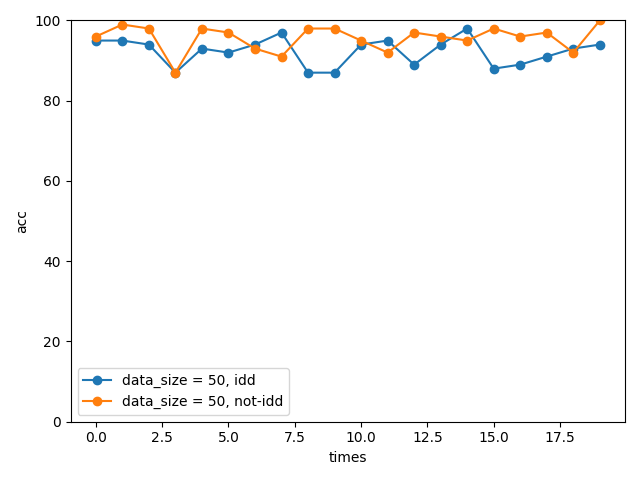
\includegraphics[width=0.6\textwidth]{img_3.png}
  \bottomcaption{贝叶斯假设}
\end{figure}
\subsection{UCI数据集测试}
使用UCI数据集测试结果如下。
\begin{figure}[htbp]
  \centering
  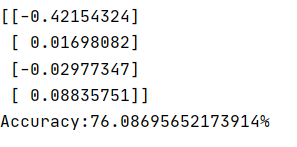
\includegraphics[width=0.6\textwidth]{img_4.png}
  \bottomcaption{UCI Haberman}
\end{figure}
将UCI数据进行可视化发现,该数据在三维空间并不线性可分,所以模型效果较差。
\begin{figure}[htbp]
  \centering
  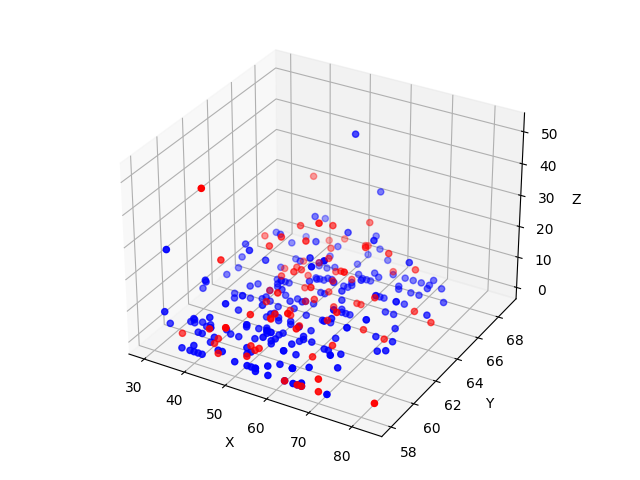
\includegraphics[width=0.6\textwidth]{img_5.png}
  \bottomcaption{UCI Data}
\end{figure}
\begin{thebibliography}{99} 
\bibitem{ref1}空中的鱼1987.逻辑回归梯度下降法详解[EB/OL].https://blog.csdn.net/lookqlp/article/details/51161640,2016-04-19.
\bibitem{ref2}阿泽.【机器学习】逻辑回归(非常详细[EB/OL].https://zhuanlan.zhihu.com/p/74874291,2019-08-01.
\end{thebibliography}

% \begin{lstlisting}[caption={一段C代码},captionpos=b]
% #include <stdio.h>
% int main (int argc, char *argv[]){
%   printf("Hello world!");
% }
% \end{lstlisting}


\end{document}
